\documentclass[11pt,twoside,romanian]{extbook}
\usepackage[T1]{fontenc}
\usepackage[utf8]{inputenc}
\usepackage{color}
\usepackage{comment}
\usepackage{times}
\usepackage[margin=1in]{geometry}
\usepackage{fancyhdr}
\usepackage{lscape}
\usepackage{float}
\usepackage{listings}
\usepackage[romanian,english]{babel}
\usepackage{amsmath}
\usepackage{amssymb,amsfonts,textcomp}
\usepackage{array}
\usepackage{hhline}
\usepackage[pdftex]{graphicx}
\PassOptionsToPackage{hyphens}{url}\usepackage[pdftitle={ANEXE - Sistemul de acces la date}, pdfauthor={RODA}, colorlinks=true, linkcolor=blue]{hyperref}

%\hypersetup{pdftex, colorlinks=true, linkcolor=blue, citecolor=blue, filecolor=blue, urlcolor=blue, pdftitle=, pdfauthor=, pdfsubject=, pdfkeywords=}
\pagestyle{fancy}
\DeclareGraphicsExtensions{.png,.gif,.jpg,.pdf}
\addto\captionsromanian{\renewcommand{\chaptername}{Sec\c{t}iunea}}

\begin{document}

\pagenumbering{arabic} 
\cfoot{\tiny{RODA}\tiny}
\fancyhead[LE,RO]{ANEXE - \leftmark}
\fancyhead[RE,LO]{\thepage}

%TODO Trebuie schimbat la fiecare Faza !

\title{ANEXA 1.\\
Faza nr. V 
cu titlul:\\
``Dezvoltare software, pachet 5: jurnalizare, modul CMS, modul management utilizatori.''
}

\author{RODA -- Arhiva Rom\^{a}n\u{a} de Date Sociale}

\date{ }

\maketitle

\newpage
\thispagestyle{plain}
\tableofcontents{}
\setcounter{page}{1}

\chapter{Modulul de management de continut (CMS)}

\section{Front-end CMS}

\include{URL-dispatching}
% Cosmin - schema si poze chiar si din docs. Spring, de ce sunt 2 dispatchere (web si json), de ce s-au structurat URL-urile in acest fel (/admin ... etc.)
% Letitia - controller '/page'

% Cosmin! e nevoie de '/admin' realizat in server

% later:  /resources/root => sa fie accesibil la:   /databrowser

\subsection{Generarea paginilor}
\label{generarea_paginilor}

Controller-ul care primeste solicitarea pentru pagina, prin intermediul unei cereri prefixate de "/page", apeleaza metoda \textbf{generatePage(url)} a serviciului \emph{RodaPageService}. 
Portiunea de URL care urmeaza lui "/page" va specifica, de fapt, o succesiune de fragmente de URL corespunzatoare unei ierarhii de pagini din baza de date. 
Pentru o pagina din baza de date, campul "url" contine, de fapt, doar fragmentul final al URL-ului paginii. 
Identificarea URL-ului integral (unic) al paginii se realizeaza prin parcurgerea bottom-up a ierarhiei, pana la pagina radacina de pe drumul respectiv. 
De regula, pagina radacina va fi "ro" sau "en", corespunzator limbii paginilor din arborescenta de sub acestea. 
De exemplu, \emph{<server>:8080/roda/page/ro/acasa} va genera si returna pagina al carei camp URL din baza de date are valoarea "acasa", si este subordonata paginii "ro". 

Metoda \textbf{generatePage(URL)} include efectuarea urmatoarelor actiuni:

\begin{enumerate}
\item{In functie de parametrul primit (URL), cauta inregistrarea corespunzatoare din tabelul de pagini al bazei de date.}
\item{Cu informatia despre pagina curenta, apeleaza metoda getLayout(cmsPage, url). Aceasta:}
\begin{itemize}
\item{regaseste continutul layout-ului in baza de date}
\item{inlocuieste toate codurile din continutul layout-ului, cu exceptia lui \emph{[[Code: PageContent]]}}
\item{returneaza continutul layout-ului.}
\end {itemize}
\item{Pe baza paginii curente si a layout-ului obtinut anterior, este apelata metoda replacePageContent(layoutContent, cmsPage). Aceasta determina daca exista codul \emph{[[Code: PageContent]]} in continutul layout-ului, iar in caz afirmativ realizeaza urmatoarele actiuni:}
\begin{itemize}
\item {regaseste continutul paginii in baza de date}
\item{inlocuieste toate codurile din continutul paginii}
\item {inlocuieste codul \emph{[[Code: PageContent]]} cu continutul paginii, astfel prelucrat.}
\end{itemize}
\end{enumerate}

\bigskip

Pagina astfel generata este trimisa, ca atribut al modelului, unui fisier show.jsp; 
in acest fisier, codul generat al paginii va corespunde sectiunii /emph{body}.
Calea (referinta) catre fisierul show.jsp este returnata de catre metoda de afisare din controller-ul de pagina, \emph{RodaPageController}.

O portiune a codului sursa al acestei metode este urmatorul:

\begin{lstlisting}[breaklines=true]
@RequestMapping(value = "/**", produces = "text/html")
public String show(HttpServletRequest request, Model uiModel) {

	String url = (String) request.getAttribute(HandlerMapping.PATH_WITHIN_HANDLER_MAPPING_ATTRIBUTE);
	..........
	String pageBody = rodaPageService.generatePage(url)[0];
	..........

	uiModel.addAttribute("pageBody", pageBody);

	return "rodapage/show";
}
\end{lstlisting}	
% Letitia

\subsection{Macro}
% Cosmin - pornind de la GoogleDocs + breadcrumbs + menu

\subsection{Thumbnails}
\label{thumbnails}

Un element important al unei interfete de administrare evoluate il constituie imaginile de tip thumbnail, care ofera mai mult control si posibilitatea unei gestiuni mai usoare a unor elemente ale interfetei grafice. Astfel, imaginile care vor fi inserate pot fi previzualizate chiar in interfata.

Aceasta functionalitate a fost implementata printr-un controller special pentru thumbnail-uri. Acesta raspunde solicitarilor corespunzatoare urmatoarelor URL-uri:

\begin{itemize}
\item{/admin/thumbnail/alias/[alias]/h/[h] - returneaza o copie a imaginii corespunzatoare aliasului [alias] taiata astfel incat sa fie un patrat cu dimensiunea [h]}

\item{/admin/thumbnail/alias/[alias]/h/[h]/w/[w] - returneaza o copie a imaginii corespunzatoare aliasului [alias] taiata astfel incat sa fie un dreptunghi cu inaltimea [h] si latimea [w]}

\item{/admin/thumbnail/alias/[alias]/x/[x] - returneaza o copie a imaginii corespunzatoare aliasului [alias] redimensionata astfel incat latimea sa fie de [x] pixeli si inaltimea dependenta de imaginea originala}

\item{thumbnail/alias/[alias]/y/[y] - returneaza o copie a imaginii corespunzatoare aliasului [alias] redimensionata astfel incat inaltimea sa fie de [y] pixeli si latimea dependenta de imaginea originala.}

\end{itemize}

Cele 4 tipuri de thumbnail-uri sunt obtinute de catre controller apeland metodele serviciului ThumbnailsService. Acest servciu utilizeaza libraria grafica imgscalr:

\url{http://www.thebuzzmedia.com/software/imgscalr-java-image-scaling-library/}, 

specificata ca dependenta Maven a aplicatiei:

\begin{lstlisting}[breaklines=true]
<dependency>
	<groupId>org.imgscalr</groupId>
	<artifactId>imgscalr-lib</artifactId>
    	<version>4.2</version> 
</dependency> 
\end{lstlisting}	

\bigskip

Thumbnail-urile corespunzatoare primelor doua URL-uri enumerate anterior presupun doua operatii asupra imaginii initiale: 
\begin{itemize}
\item {o operatie de tip crop, in urma careia se obtine cel mai mare dreptunghi, care pastreaza fie latimea, fie inaltimea imaginii initiale, cu proprietatea ca este proportional cu dimensiunile imaginii cerute}
\item{o operate de tip scale asupra imaginii obtinute anterior, astfel incat aceasta sa fie adusa la dimensiunea ceruta.}
\end{itemize}  

Thumbnail-urile corespunzatoare ultimelor doua URL-uri enumerate anterior presupun doar o operatie de tip scale asupra imaginii initiale.

\bigskip

Metodele principale ale servicului ThumbnailsService, care sunt invocate si de catre celelalte metode oferite de acest serviciu, sunt urmatoarele:

\begin{itemize}
\item{generateThumbnailByHeightAndWidth(url, alias, height, width) - primeste ca parametri: URL-ul fata de care este relativ URL-ul imaginii initiale, alias-ul fisierului imagine (in functie de acesta, fisierul va fi gasit in baza de date), precum si dimensiunile noii imagini. Metoda determina dimensiunea imaginii care se incadreaza optim in imaginea initiala, astfel incat sa fie proportionala cu dimensiunile cerute, apoi utilizeaza una dintre metodele de redimensionare (resize) ale librariei imgscalr pentru a obtine thumbnail-ul dorit.)}
\item{generateThumbnailProportional(url, alias, height, width) - parametrii sunt similari celor ai metodei anterioare. Aceasta metoda va fi apelata cu valoarea null pentru unul dintre parametrii corespunzatori dimensiunii, urmand ca imaginea obtinuta sa respecte dimensiunea nenula, cealalta dimensiune fiind determinata proportional cu aceasta, relativ la dimensiunile imaginii originale.}
\end{itemize}

\bigskip

Imgscalr este o librarie pentru scalare de imagini, care se bazeaza atat pe tehnicile eficiente oferite de pachetul Java2D (referitoare la accelerarea hardware de pe toate platformele), cat si pe implementarea unui algoritm optimizat de scalare incrementala. 
Alegerea acestei librarii spre a fi utilizata in proiect a avut drept motivatie simplitatea si eficienta realizarii operatiilor necesare obtinerii thumbnail-urilor pentru interfata de administrare. Un aspect important al acestei optiuni a avut in vedere faptul ca libraria imgscalr permite redimensionarea rapida a imaginilor.
Libraria imgscalr constituie, de fapt, o multime  de operatii grafice optimizate. Utilizarea acesteia in cadrul metodelor din serviciul ThumbnailsService a presupus apeluri statice precum cel din urmatorul exemplu:

\begin{lstlisting}[breaklines=true]
BufferedImage resultImage = Scalr.crop(bufferedImage, (int) x, (int) y, (int) fitWidth, (int) fitHeight, (BufferedImageOp[]) null);
\end{lstlisting}	

Imaginea (obtinuta relativ la URL-ul curent si pe baza aliasului fisierului respectiv) este trimisa librariei, pentru a fi taiata relativ la punctul de coodonate (x, y), astfel incat sa se obtina o imagine de dimensiuni fitWidth, fitHeight.

Imaginea obtinuta anterior poate fi apoi redimensionata cu ajutorul librariei imgscalr, astfel:

\begin{lstlisting}[breaklines=true]
resultImage = Scalr.resize(resultImage, width, height, (BufferedImageOp[]) null);  
\end{lstlisting}	





% Letitia

\subsection{Cache} 
%Cosmin - ehcache, de ce aceasta solutie, scalabilitate, configurare manager si cache-uri individuale, implementare

\section{Administrare CMS}

Administrarea modulului de management de continut trebuie sa permita
efectuarea tuturor operatiilor de modificare, adaugare si intretinere
a continutului site-ului care prezinta informatia stocata de RODA.
Acest component este deosebit de important pentru ca aici se construieste
informatia pe care o veede orice vizitator sau utilizator al arhivei
care avveseaza pagina acesteia. Chiar daca o parte insemnata din informatia
transmisa prin acest site este produsa si administrata cu ajutorul
altor module (ex: databrowser), chiar si aceasta va trebui sa fie
integrata intr-o pagina web iar aceasta integrare se face in modulul
de administrare a continutului. 

Administrarea continutului presupune operatii de vizualizare, modificare
si stergere a urmatoarelor tipuri de informatie: layout, snippet,
fisiere si pagini, dispuse in structura unei pagini ca in figura urmatoare:

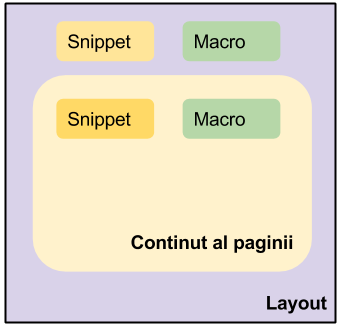
\includegraphics[width=7cm]{cms/roda-page}


\subsection{Administrarea layout-urilor}

Layout-ul reprezinta ansamblul de elemente html, css si javascript
care inconjoara continutul fiecarei pagini. Astfel, layoutul este
un fel de sablon care se aplica asupra continutului paginii in procesul
de constructie a acesteia. Existenta layoutului permite separarea
elementelor de design de elementele de continut, in mare parte a cazurilor,
modificarea informatiei afisata in paginile RODA se va putea face
fara a afecta elementele de design datorita existentei conceptului
de layout. 

Lista layouturilor si proprietatile acestora se pot vedea impreuna
pe acelasi ecran pentru a putea identifica rapid ce este de modificat,
daca este cazul. De asemenea, fiecare layout este insotit de o lista
a paginilor care il folosesc, pentru a se vedea ce pagini vor fi afectate
de eventualele modificari efectuate. 

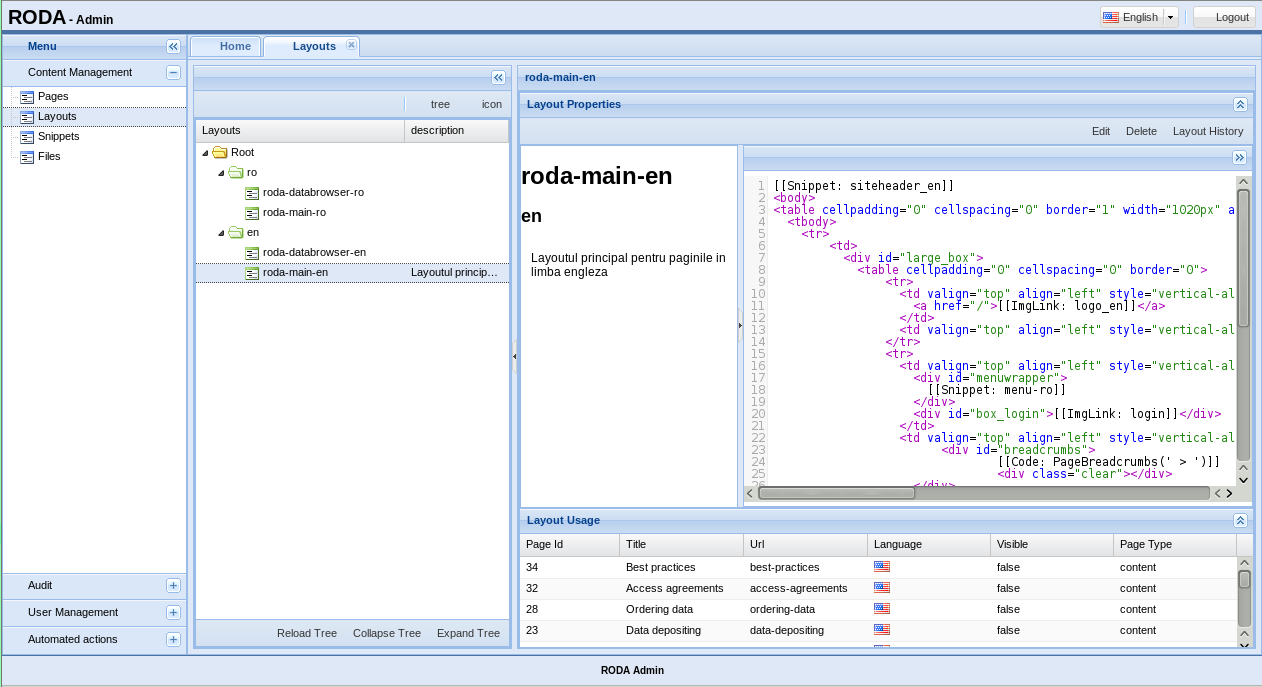
\includegraphics[width=15cm]{cms/backend/layout/cmslayout1}

Pentru a putea ordona mai usor colectia de layouturi acestea pot fi
grupate in grupuri. Grupurile sunt dispuse intr-o structura arborescenta,
ca un fel de foldere. In panoul din stanga ecranului se vede structura
ierarhica alcatuita din grupuri si layouturile prezente in fiecare
din acestea. La selectia unui element din arborele principal, in partea
dreapta a ecranului sunt incarcate elementele acestuia, nume, descriere,
continut, paginile utilizate. In cazul in care este selectat un folder,
panourile dedicate continutului si paginilor se retrag pentru ca nu
sunt necesare. 

Intrucat layouturile constau in principal din cod HTML, a fost implementat
un component special pentru vizualizarea acestuia, component care
coloreaza anumite parti ale textului. 

Operatiile de modificare, stergere, sunt disponibile atat din bara
din partea dreapta a ecranului cat si prin folosirea meniurilor contextuale
disponibile la click pe butonul drept al mouseului, asa cum se poate
vedea in figura urmatoare:

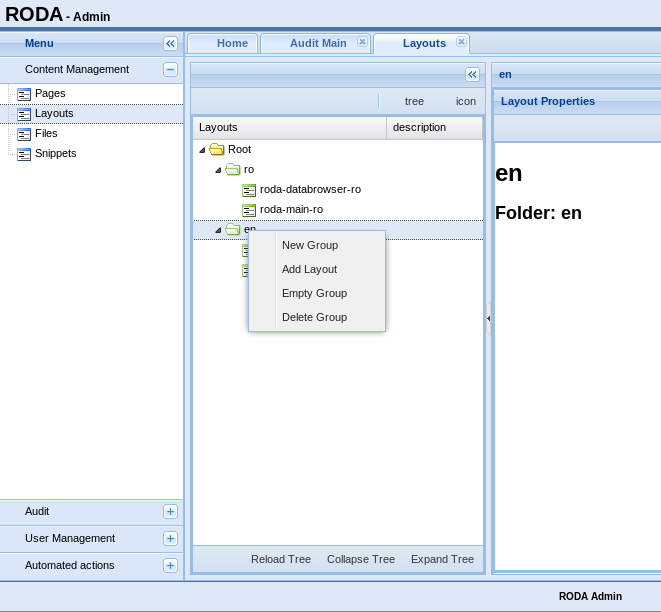
\includegraphics[width=10cm]{cms/backend/layout/cmslayout2}

Modificarea grupurilor presupune schimbarea denumirii precum si eventual
a descrierii lor, ca si repozitionarea lor pe ierarhia acestora. Aceste
operatii sunt disponibile prin intermediul unui dialog modal care
se poate vedea in figura urmatoare:

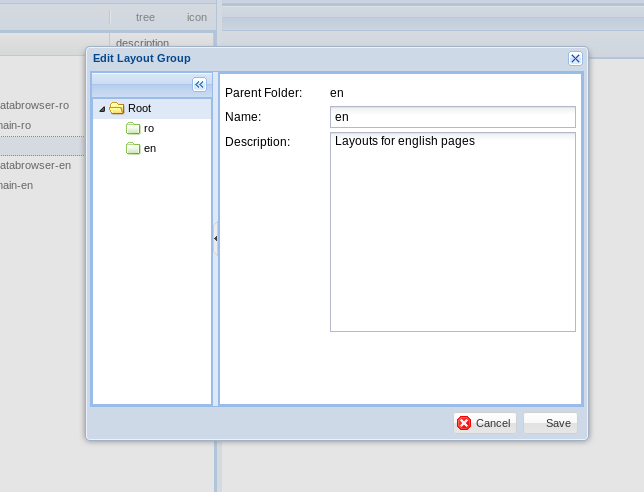
\includegraphics[width=10cm]{cms/backend/layout/cmslayout4}

In partea stanga a dialogului se poate vedea ierarhia de grupuri.
Grupul curent este direct subordonat radacinii. Daca se doreste mutarea
acestuia in alt grup, se selecteaza noul parinte din aceasta coloana.
In partea dreapta se pot modifica numele si descrierea grupului.

Operatiile de modificare ale layouturilor sunt de asemenea disponibile
prin intermediul unui dialog modal care arata ca in figura urmatoare:

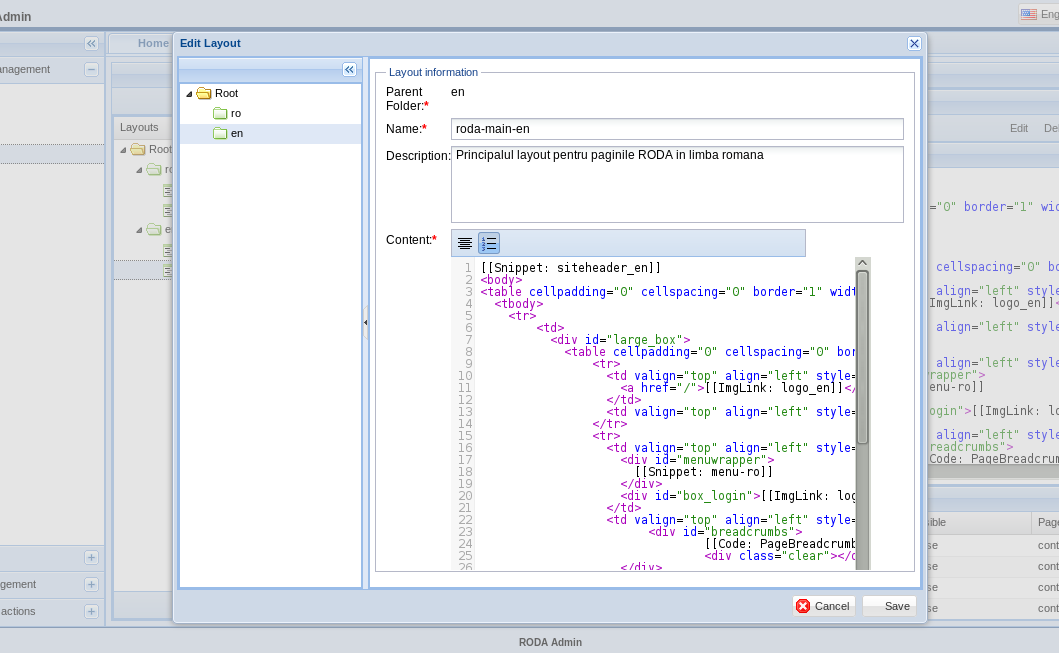
\includegraphics[width=15cm]{cms/backend/layout/cmslayout5}

Coloana din partea stanga este de asemenea menita selectiei grupului
in care se gaseste layoutul curent. Coloana din partea dreapta permite
modificarea numelui, descrierii precum si a continutului layoutului.
Intrucat in marea majoritate a cazurilor layoutul contine in principal
cod HTML, a fost implementat un editor special care permite o vizualizare
mult mai clara a elementelor de continut si adauga numerotarea liniilor. 

Interfata de management al layouturilor permite multiple variante
de aranjare pentru a putea acomoda toate tipurile de rezolutie ale
monitoarelor, fara a forta afisarea unei cantitati mai reduse de continut.
Astfel, diversele panouri ale acesteia pot fi minimizate, asa cum
se poate vedea in figura urmatoare:

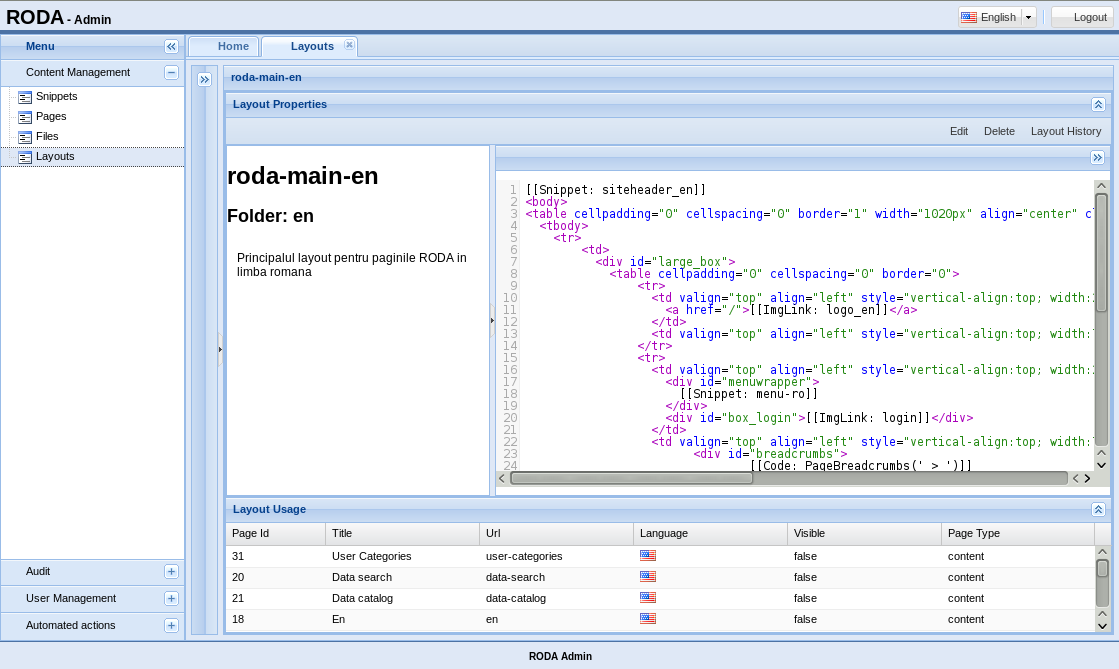
\includegraphics[width=15cm]{cms/backend/layout/cmslayout7}

Se poate observa ca lista grupurilor si a layouturilor a fost redusa
obtinandu-se astfel un spatiu mult mai mare pentru a putea urmari
continutul si lista paginilor care utilizeaza layoutul. In egala masura,
daca operatorul doreste sa consulte lista paginilor utilizate pe o
suprafata mai mare, proprietatile layoutului (nume, descriere si continut)
pot fi de asemenea minimizate, lista de pagini care folosesc layoutul
curent umpland intreaga zona, dupa cum se poate vedea in figura urmatoare:

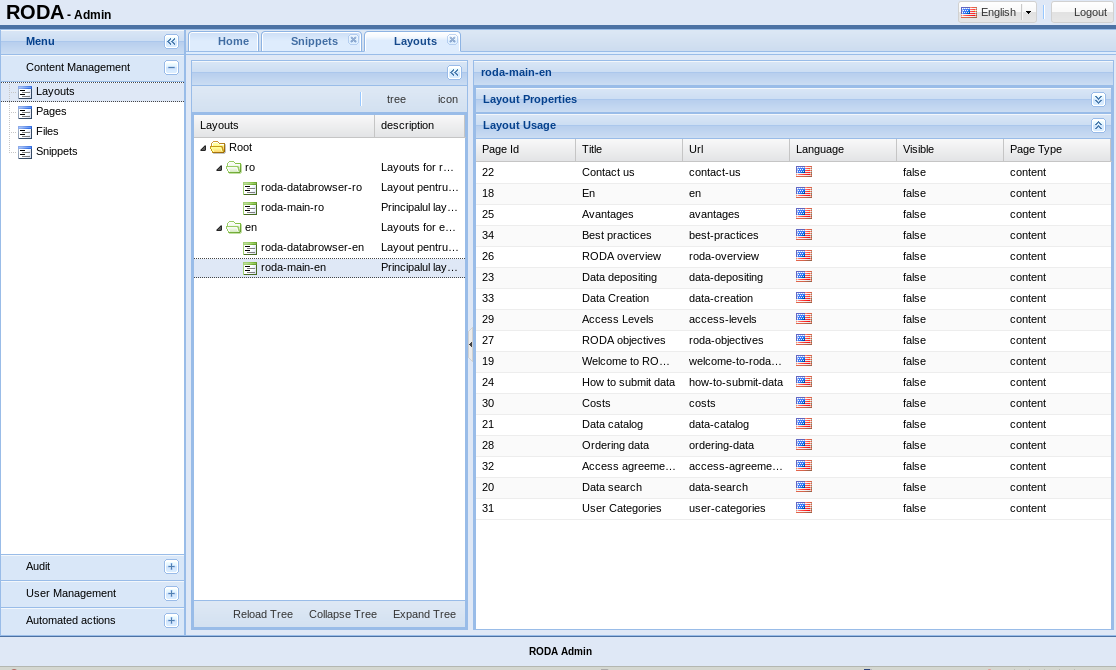
\includegraphics[width=15cm]{cms/backend/layout/cmslayout8}

Structurile arborescente sunt foarte utile in organizarea informatiei
dar in anumite situatii, cand devin prea stufoase, acestea pot fi
dificil de utilizat. Pentru situatiile in care operatorul poate identifica
layoutul care il intereseaza fara sa traverseze intreaga structura
arborescenta, panoul arborescent poate fi inlocuit cu un panou tabelar,
panou in care nu apar si grupurile, dupa cum se vede in figura urmatoare:

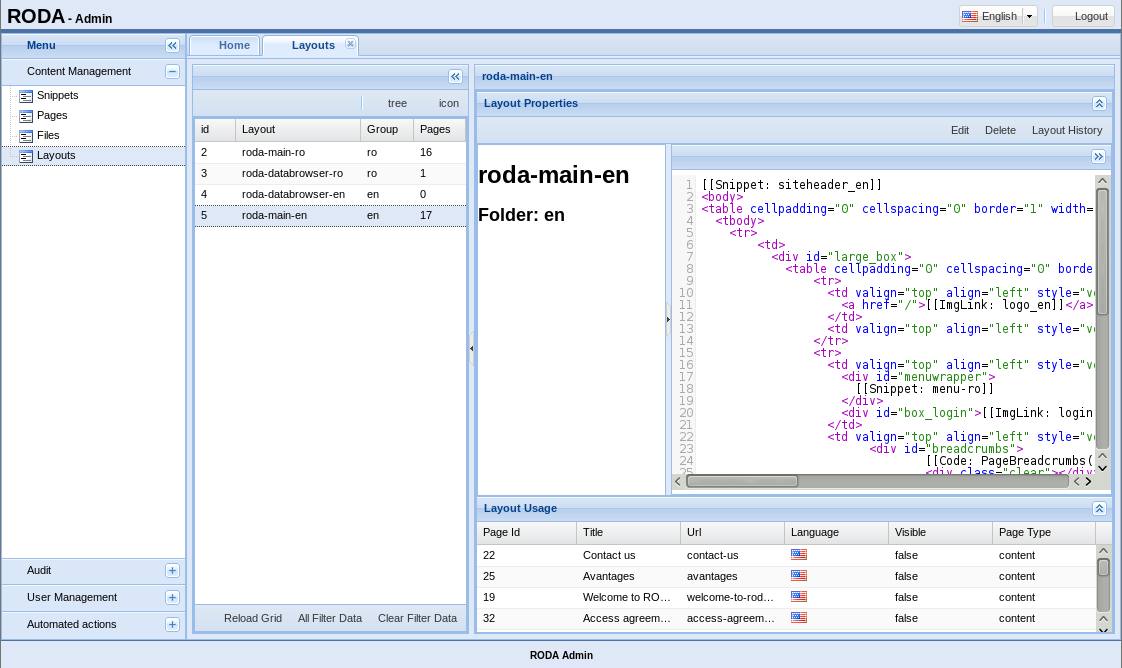
\includegraphics[width=15cm]{cms/backend/layout/cmslayout9}

Ca si in cazul panoului arborescent, la selectia unui layout din tabelul
din stanga, acesta va fi incarcat in panoul din dreapta unde vor fi
disponibile toate optiunile care puteau fi accesate si in cazul panoului
arborescent. 

Atat panoul arborescent cat si cel tabelar permit operatii de sortare
si filtrare care permit navigarea mai usoara prin listele stufoase:

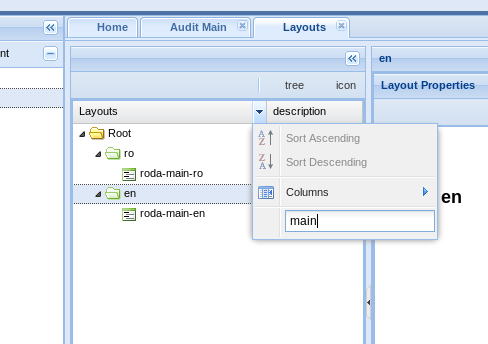
\includegraphics[width=10cm]{cms/backend/layout/cmslayout10}


\subsection{Administrarea snippet-urilor}

Orice informatie prezentata pe web prin folosirea standardelor obisnuite
presupune, de obicei, foarte multe fragmente repetabile. Fragmente
care se gasesc nemodificate in layouturi sau in pagini si a caror
includere directa ar determina cresterea continutului acestora si
urmarirea mult mai dificila a informatiei. De aceea au fost implementat
submodulul de administrare a snippet-urilor, care sunt astfel de fragmente
reutilizabile pe care editorii le au la dispozitie oricand prin intermediul
unul macro special dezvoltat pentru acestea, {[}{[}Snippet{]}{]}.
Trebuie mentionat ca, spre deosebire de celelalte elemente de continut
prezentate aici, un snippet poate include alte snippeturi.

Interfata de administrare a snippeturilor este, ca si cea prezentata
mai sus, dispusa intr-un singur ecran cu elemente interschimbabile,
destul de asemenatoare cu cea de la layouturi, evident, cu particularitati
specifice:

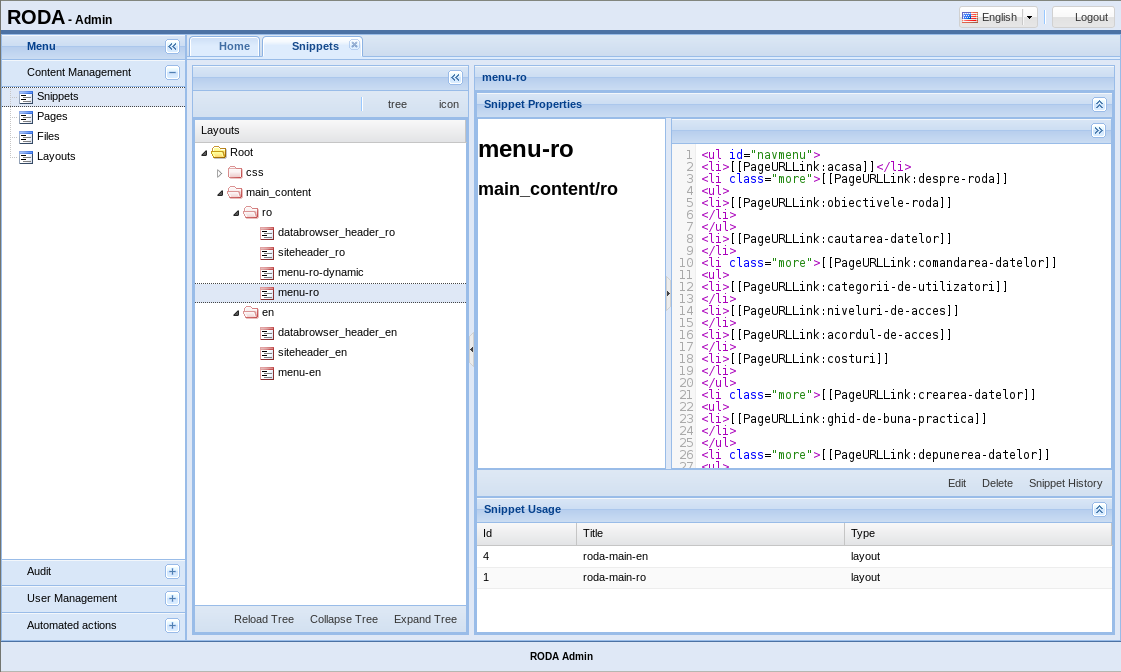
\includegraphics[width=15cm]{cms/backend/snippet/snippet1}

Ca si layoutile, snippet-urile sunt distribuite intr-o structura arborescenta
de grupuri. Acestea sunt utile exclusiv pentru ordonare, mutarea unui
snippet dintr-un grup intr-altul nu afecteaza elementele de continut
superioare care il utilizeaza. Ca si in cazul layouturilor, se poate
observa ca interfata contine un arbore de grupuri cu snippet-urile
corespunzatoare in partea stanga, insotit de un panou de detalii in
partea dreapta in care sunt prezentate proprietatiile elementului
selectat in panoul din stanga. Si aici exista o sectiune speciala
pentru utilizarea snippetului, care prezinta lista elementelor de
continut in care a fost apelat. Acestea pot fie layouturi, pagini
sau chiar alte snippet-uri.

Modificarea grupurilor se face prin intermediul unui dialog modal
care permite atat selectia parintelui in ierarhia arborescenta a grupurilor
cat si modificarea numelui sau a descrierii acestuia:

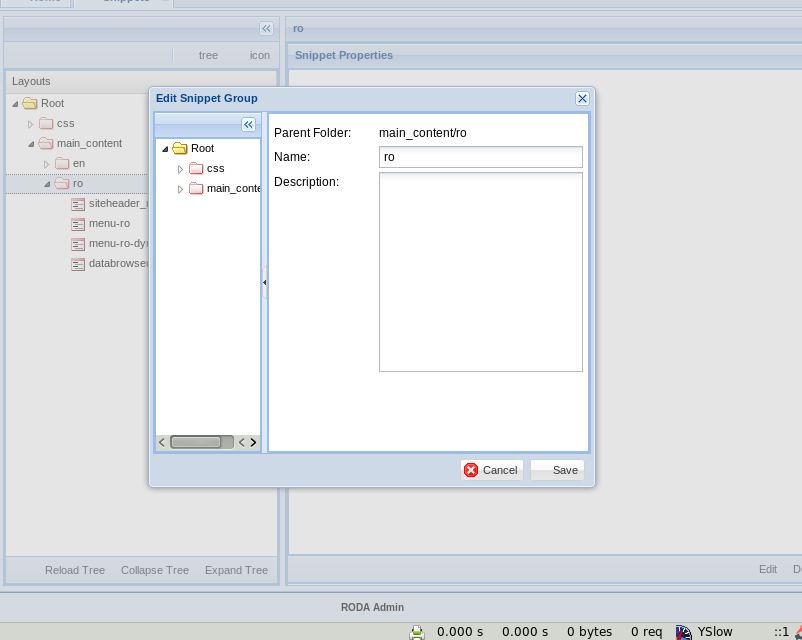
\includegraphics[width=12cm]{cms/backend/snippet/snippet2}

Modificarea snippetului (sau adaugarea unui snippet nou) se face tot
prin intermediul unui dialog modal care contine o structura similara
de panouri, unul in partea stanga pentru alegerea grupului din care
va face parte acesta si unul in partea dreapta unde se pot modifica
numele sau continutul acestuia:

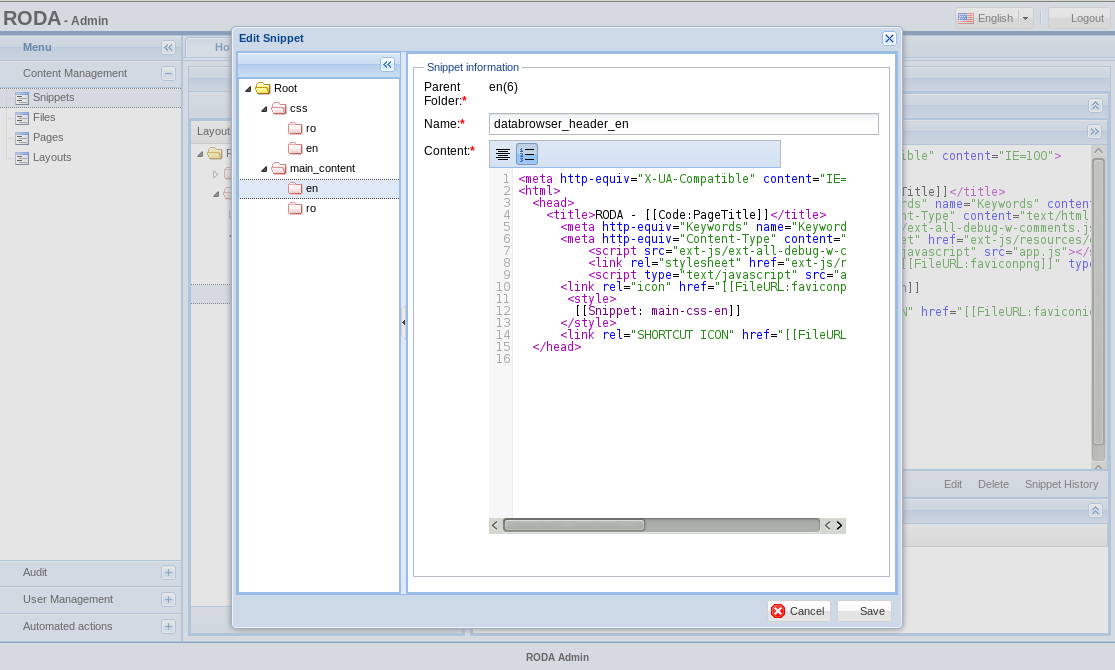
\includegraphics[width=15cm]{cms/backend/snippet/snippet3}

Si in cazul snippet-urilor este de asteptat ca in mare masura acestea
sa contina elemente specifice limbajului internetului, HTML, CSS,
javascript. De aceea, a fost implementat si aici acelasi editor care
evidentiaza elementele standard prin culori diferite. 

Panoul de administrare a snippet-urilor permite aceeasi flexibilitate
ca si cel de la layout-uri in privinta aranjarii componentelor pentru
diferite moduri de lucru sau rezolutii de monitoare. In figura urmatoare
se vede cum elementele descriptive ale snippetului au fost minimizate
ramanand intreg spatiu la dispozitia listei de elemente care utilizeaza
snippet-ul curent:

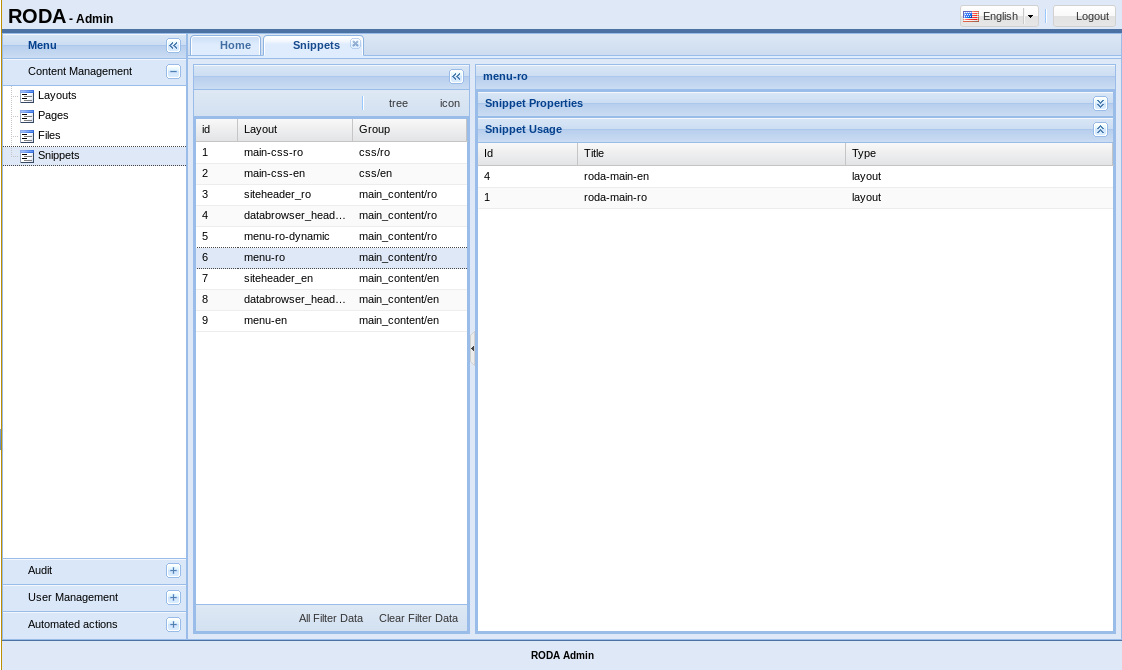
\includegraphics[width=15cm]{cms/backend/snippet/snippet5}

Pentru cazurile in care operatorul prefera ca lista de snippeturi
sa fie tabelara, ca si interfata pentru layouturi, si aceasta ofera
posibilitatea de a schimba lista arborescenta, asa cum se vede in
imaginea urmatoare:

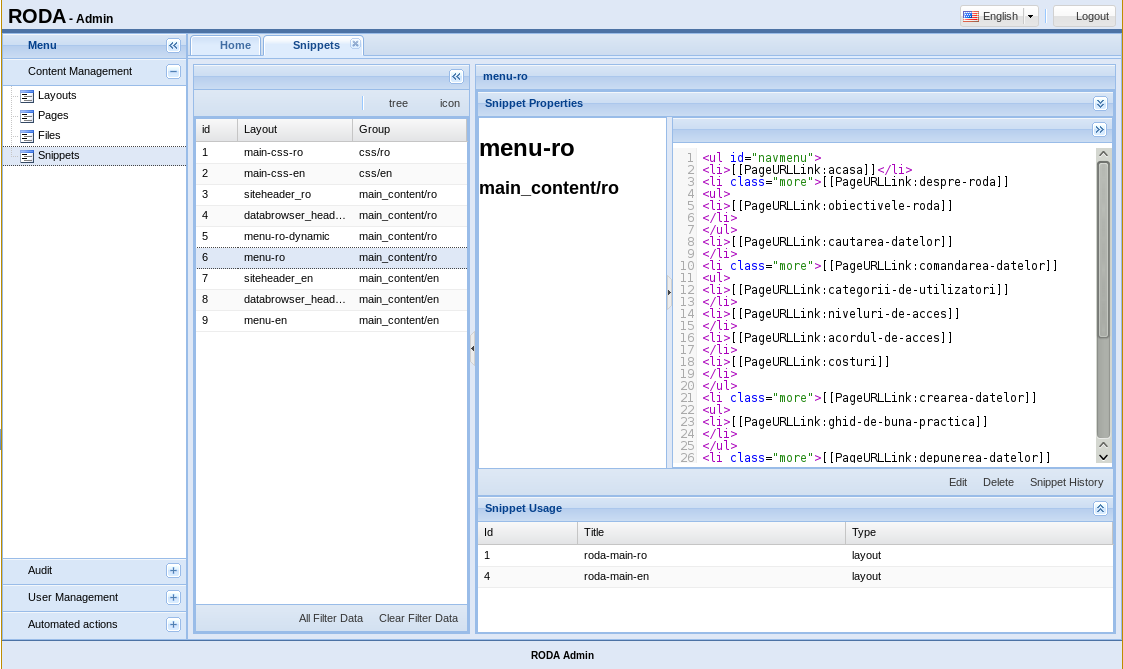
\includegraphics[width=15cm]{cms/backend/snippet/snippet6}

Si aici, elementele selectate in panoul tabelar sunt disponibile in
panoul de detalii. 

Modificarile se pot apela si aici din butoanele disbonibile la baza
panourilor cat si din meniuri contextuale disponibile la apelarea
butonului din dreapta al mouseului. 

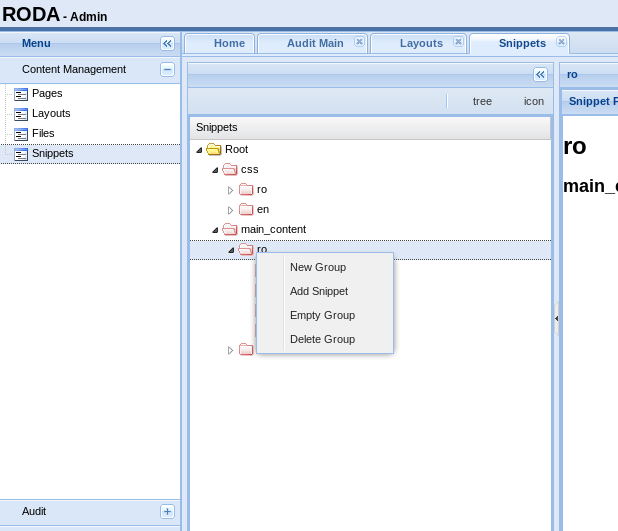
\includegraphics[width=15cm]{cms/backend/snippet/snippet7}


\subsection{Administrarea fisierelor }

Toate site-urile contin, pe langa fragmente de text sau HTML si imagini
sau alt fel de documente (pdf, doc, etc.). Ca si celelalte tipuri
de continut care se vor folosi in interfata RODA, si acestea vor fi
supuse diferitelor tipuri de modificari. Pentru aceasta, a fost implementata
o sectiune speciala a modulului CMS care permite operatiile cu fisiere. 

Arhiva RODA va contine mai multe tipuri de fisiere. O parte dintre
acestea sunt folosite doar pentru CMS (imagini care apar pe site,
documente utile vizitatorilor cum ar fi acorduri de acces si altele)
iar o parte vor fi componente ale datelor sociologice pe care RODA
le arhiveaza. Modulul prezentat in continuare NU are acces la cele
din urma, serverul are doua zone complet independente de stocare a
fisierelor iar acest modul poate accesa doar zona destinata operatiilor
de modificare a informatiei WEB. 

Panoul de administrare a fisierelor este prezentat intr-o singura
pagina, cu elemente interschimbabile. 

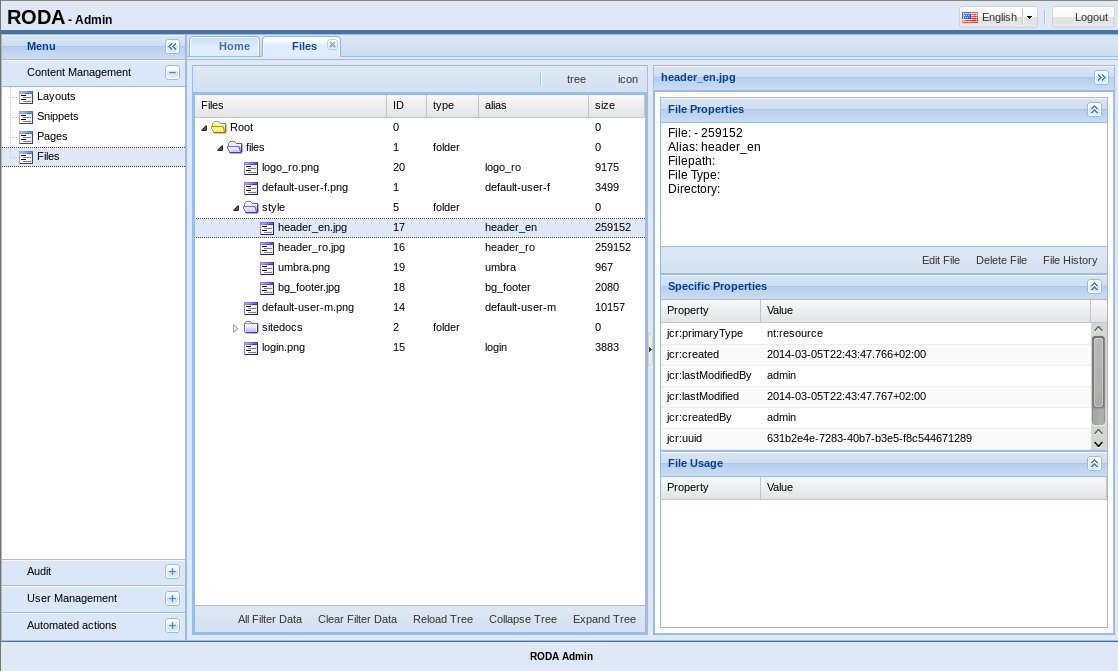
\includegraphics[width=15cm]{cms/backend/files/files1}

Fisierele sunt grupate pe foldere, la fel ca si in sistemele de fisiere
clasice. Aici scopul gruparii pe foldere este insa mai putin critic,
prin stocarea lor duala, atat intr-un repository dedicat cat si ca
referinte in baza de date, nu este nevoie de parcurgerea arborelui
de directoare pentru identificarea unui fisier, asa cum cer sistemele
de fisiere clasice. Astfel, aici fisierul va putea fi apelat direct,
la fel ca in cazul snippet-ului. Pentru a face posibil acest lucru,
fiecare fisier are un alias, un nume alternativ, diferit de numele
sau propriu-zis. In cele mai multe situatii fisierele vor fi apelate
din alte elemente de continut prin intermediul acestui alias care
este unic. 

La selectia unui fisier din panoul din stanga apar informatiile de
detaliu ale acestuia. Acestea sunt impartite in trei zone. Zona de
proprietati comune (proprietati pe care le va avea orice fisier) cum
ar fi aliasul prezentat mai sus, pozitia sa in structura de foldere,
dimensiune, etc. Zona de proprietati specifice contine elementele
specifice tipului de fisier selectat precum si informatii tipice repositoriului
JackRabbitt in care este stocat acesta. In cel de-al treilea panou,
dedicat utilizarii fisierului se vad toate elementele de continut
(pagini, layout-uri, snippet-uri, etc.) care au apelat acest fisier
si l-au inclus in structura lor. 

Ca si in cazurile precedente, exista situatii in care structura de
foldere mai mult incurca decat ajuta. Datorita modului dual de stocare,
se poate si aici inlocui panoul arborescent cu unul tabelar in care
fisierele sunt prezentate impreuna:

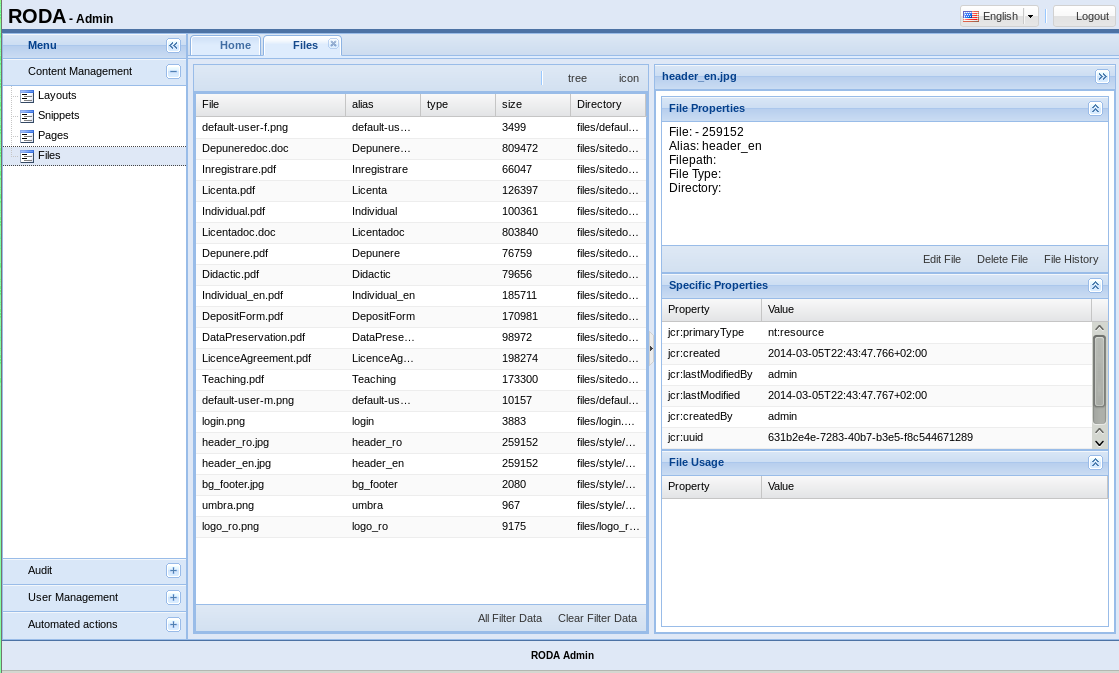
\includegraphics[width=15cm]{cms/backend/files/files2}

Ecranul permite modificarea fisierelor si a folderelor, adaugarea
acestora, stergerea lor precum si mutarea lor in alta parte a structurii
arborescente. 

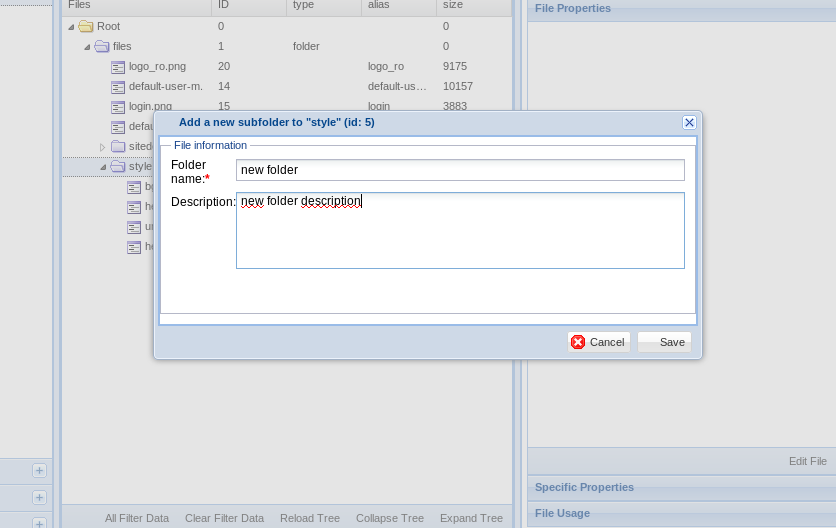
\includegraphics[width=14cm]{cms/backend/files/files3}

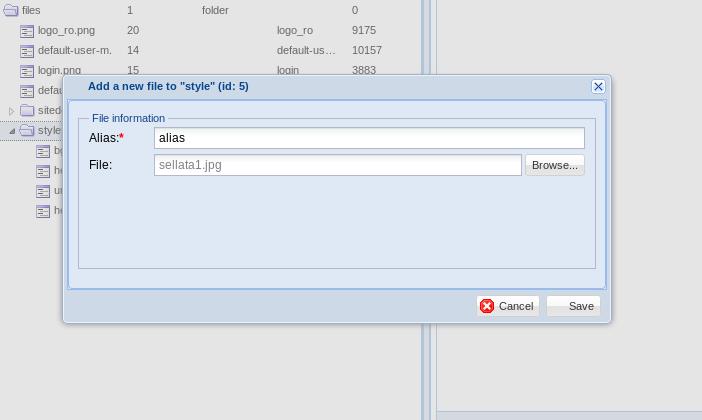
\includegraphics[width=8cm]{cms/backend/files/files4}


\subsection{Administrarea paginilor}

Paginile sunt cele mai importante elemente de continut. Paginile sunt
de fapt cele care sunt apelate de catre utilizatori prin intermediul
URL-urilor si cele care poarta informatia. Spre deosebire de elementele
prezentate mai sus, unde ierarhia era doar un mod de ordonare fara
impact direct asupra vizitatorilor, ierarhia paginilor este importanta
pentru ca ea determina adresa finala a acestora. 

Administrarea paginilor se face dintr-un singur ecran cu elemente
care se pot schimba intre ele, ca si la elementele anterioare. 

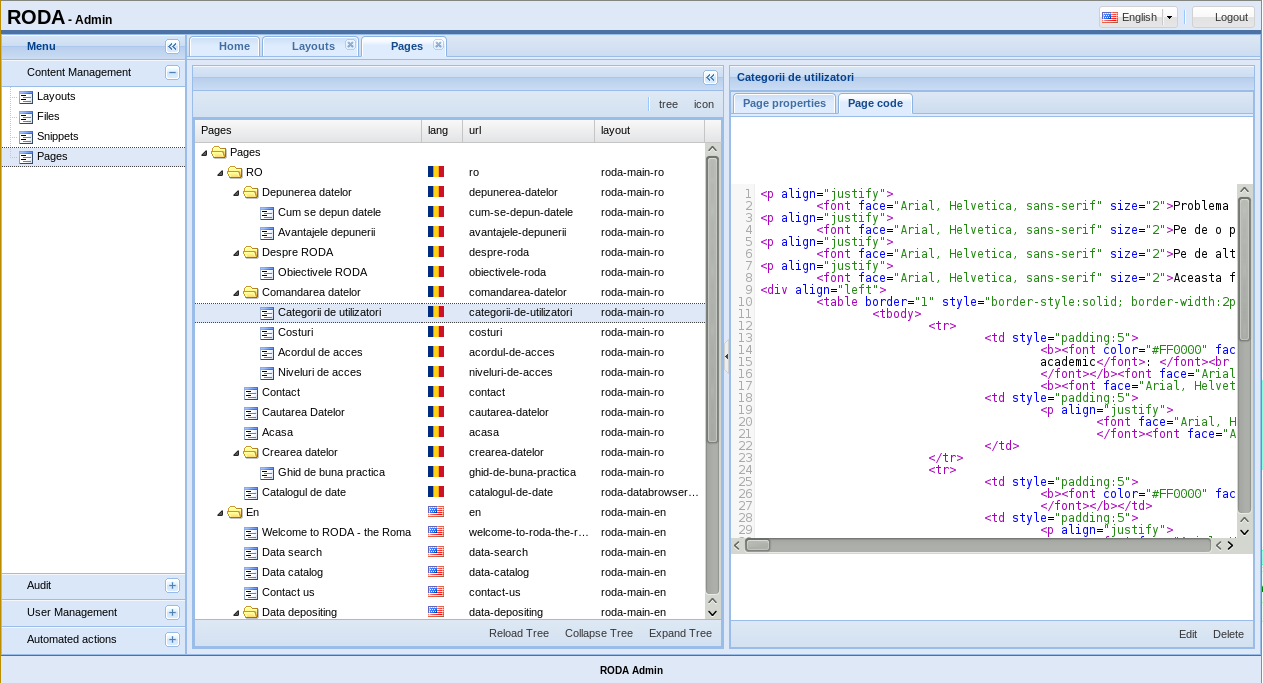
\includegraphics[width=15cm]{cms/backend/pages/cmspages1}

In partea stanga a ecranului se vede arborele de pagini, impreuna
cu o serie de informatii ajutatoare cum ar fi limba, url-ul acesteia
sau layoutul pe care il utilizeaza. La selectarea uneia dintre paginile
din structura, in partea din dreapta a ecranului se incarca proprietatile
acesteia. Panoul de proprietati contine doua taburi, unul care prezinta
codul paginii in limbaj HTML, celalalt care prezinta proprietatile
paginii si imaginea acesteia asa cum se va vedea in site, fara insa
sa se adauge si layoutul corespunzator:

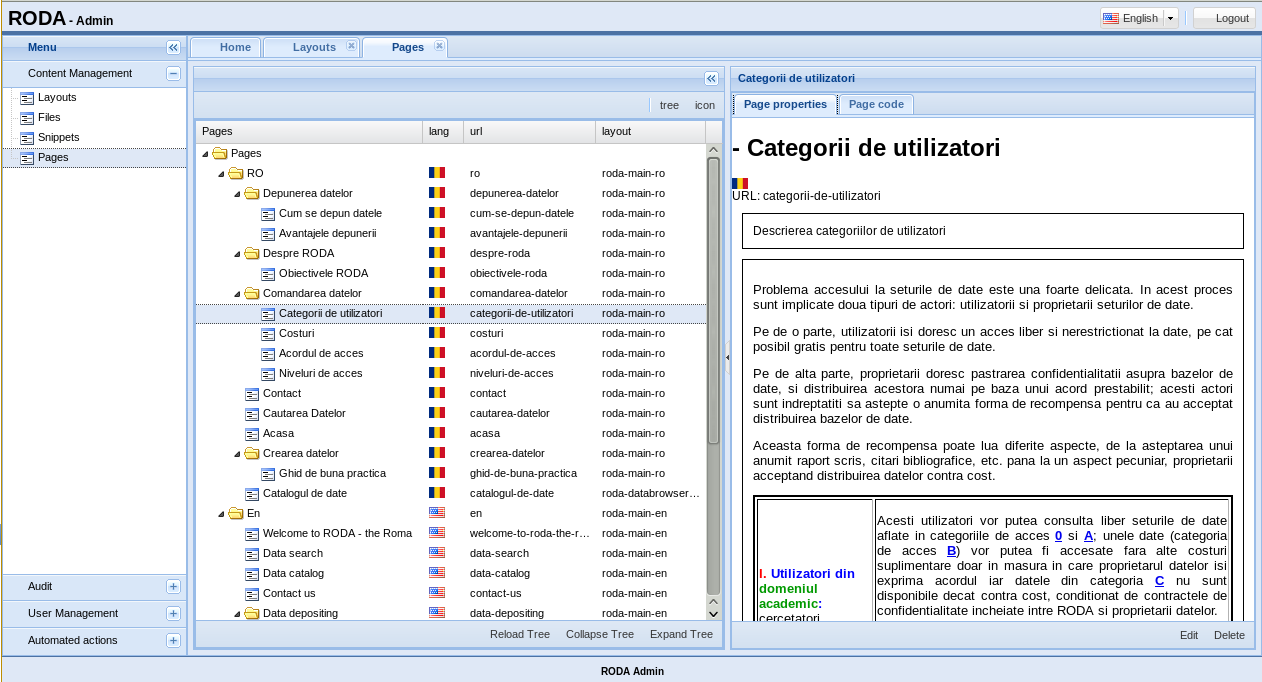
\includegraphics[width=15cm]{cms/backend/pages/cmspages2}

Editarea proprietatilor paginii, sau adaugarea unei pagini noi se
face prin intermediul unui dialog modal care permite reasezarea paginii
in structura precum si modificarea proprietatilor acesteia:

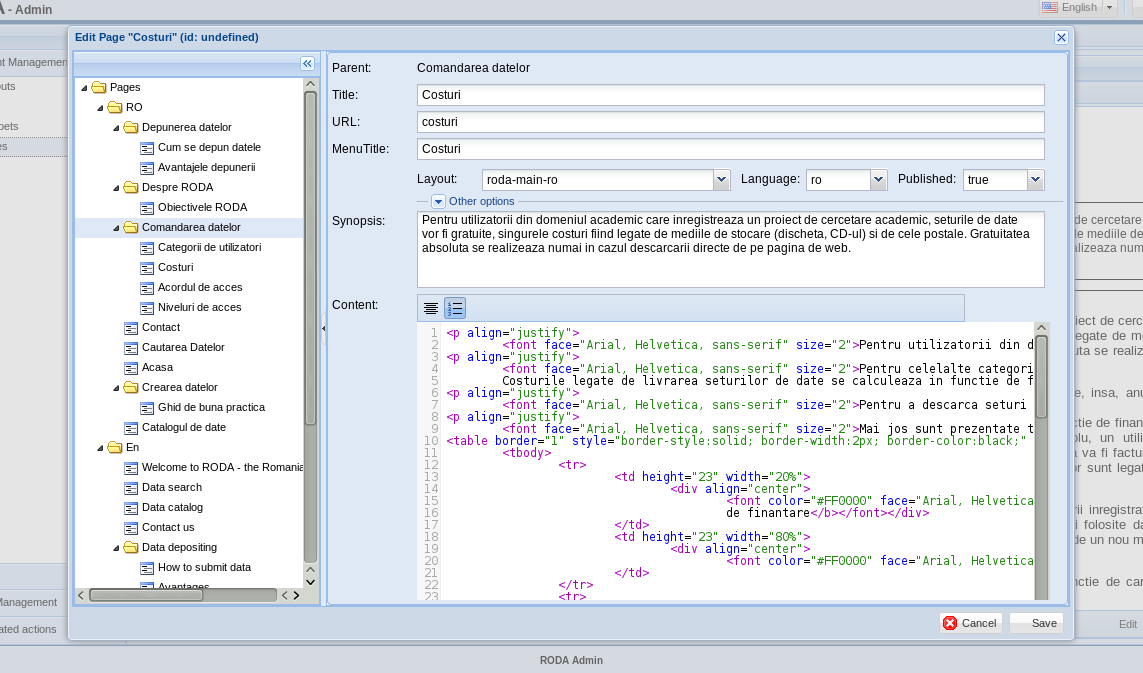
\includegraphics[width=15cm]{cms/backend/pages/cmspages3}

Ca si pentru celelalte elemente de continut, si in cazul paginii a
fost implementat acelasi editor special pentru evidentierea elementelor
HTML si css. Cantitatea semnificativ mai mare de optiuni necesare
pentru precizarea proprietatilor unei pagini a facut necesara introducerea
unui panou suplimentar care contine optiuni pe care operatorii nu
au nevoie sa le modifice frecvent:

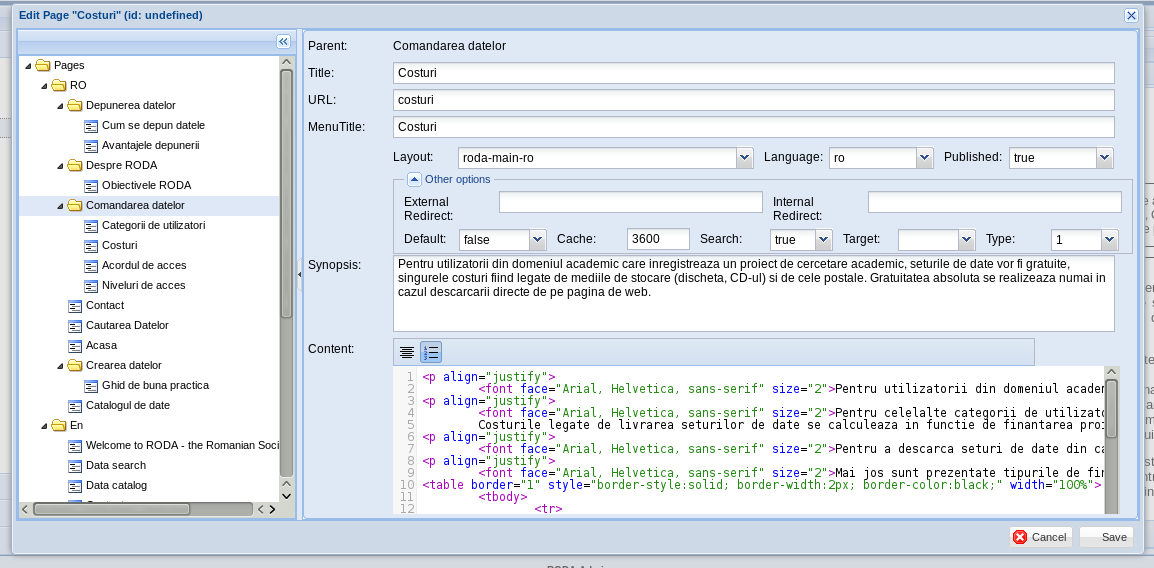
\includegraphics[width=15cm]{cms/backend/pages/cmspages6}

Ca si in cazul elementelor de mai sus, exista o serie de componente
ajutatoare care permit sortarea si filtrarea paginilor pentru gasirea
mai usoara a acestora:

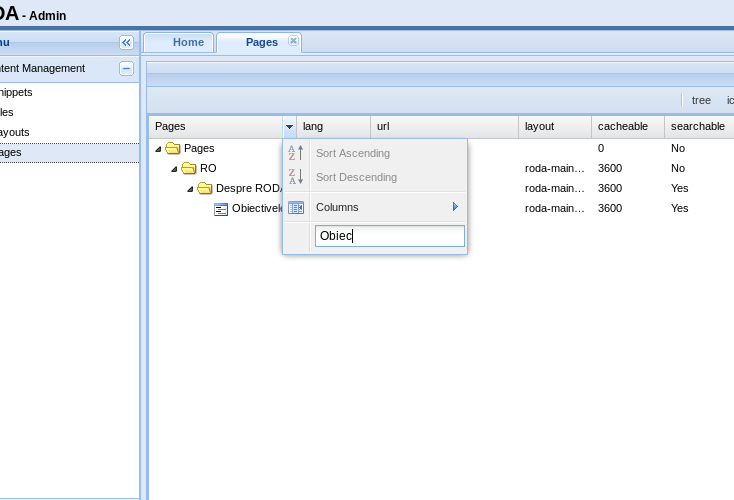
\includegraphics[width=10cm]{cms/backend/pages/cmspages5}

% Sorin - interfata de administrare a CMS

\chapter{Modulul de management al utilizatorilor}
Administrarea utilizatorilor este foarte importanta, orice aplicatie
este construita pentru utilizatorii sai. Elementele necesare in cazul
specific al RODA sunt cele clasice: posibilitatea trecerii in revista
a utilizatorilor sistemului, posibilitatea invalidarii acestora daca
este cazul, posibilitatea asocierii acestora la diferite grupuri pentru
a li se atribui diferite seturi de drepturi, posibilitatea modificarii
datelor personale ale acestora in cazul in care este nevoie, etc. 

RODA nu va avea (si nu are nevoie) de un sistem avansat de interactiune
sociala intre utilizatori, acestia nu trebuie sa se poata invita unii
pe ceilalti sa faca parte din diferite grupuri si nici nu vor avea
liste de prieteni sau alt fel de asocieri arbitrare. 

Administrarea utilizatorilor se va face intr-un ecran dedicat, de
unde vor fi accesibile toate operatiile necesare. 

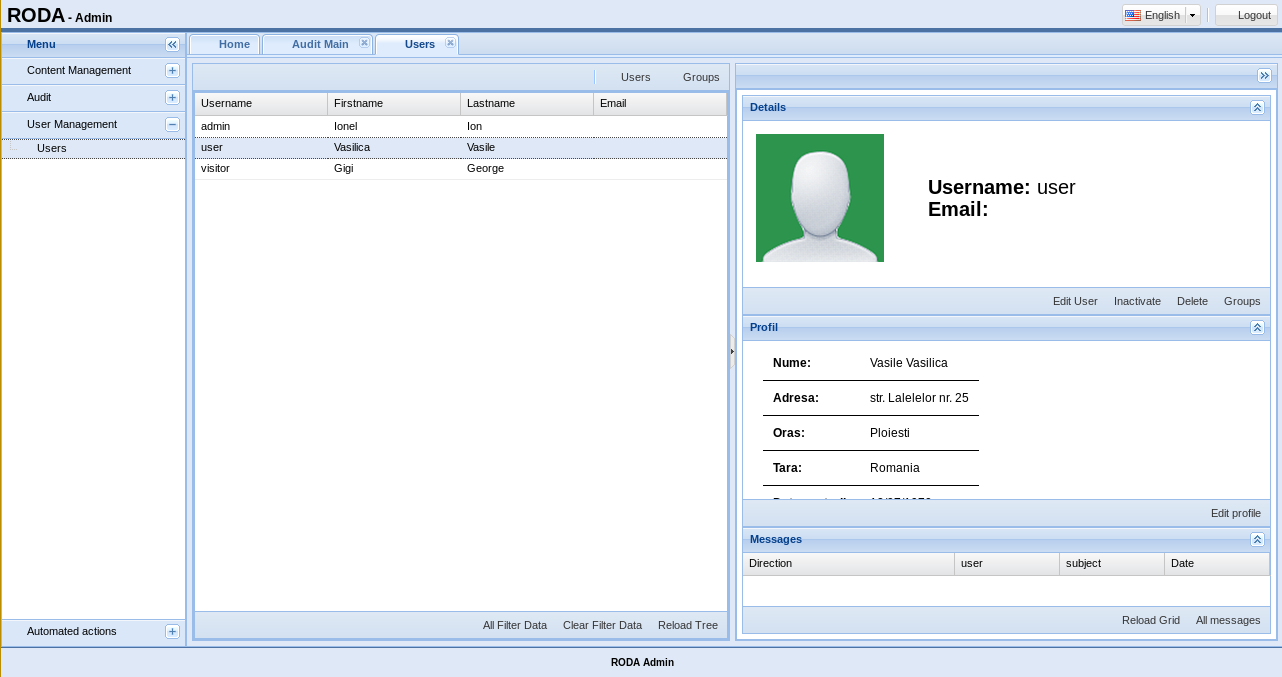
\includegraphics[width=15cm]{user/user1}

Zona de detalii este impartita in trei segmente - unul care contine
informatiile fundamentale ale utilizatorului (nume, email, etc.),
una care contine informatiile de profil ale acestuia (adresa, data
nasterii) si una care contine lista de mesaje pe care acesta le-a
primit de la sistem sau de la administratori. 

Mesajele trimise utilizatorilor de catre sistem sau de catre administratori
sunt importante - ele contin informatii pe care utilizatorul trebuie
sa le stie. Este important pentru administratori sa stie daca un anumit
utilizator cunoaste aceste informatii, pentru a rezolva eventuale
probleme pe care acesta le poate avea in utilizarea sistemului.

Ca lista de utilizatori, administratorii pot apela din ecranul din
partea stanga si lista de grupuri. 

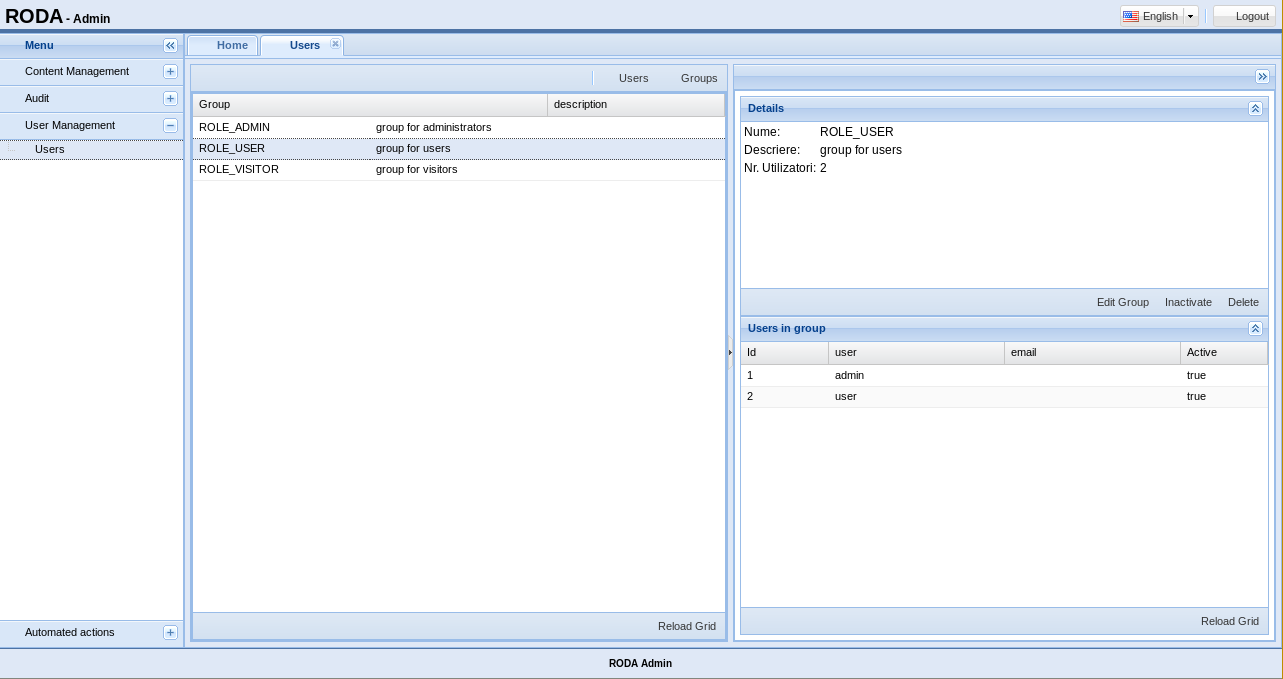
\includegraphics[width=15cm]{user/user4}

Detaliile disponibile in cazul unui grup sunt mai putine - numele
si descrierea acestuia precum si lista utilizatorilor care fac parte
din grupul curent. 

Modulul permite de asemenea adaugarea sau modificarea utilizatorilor:

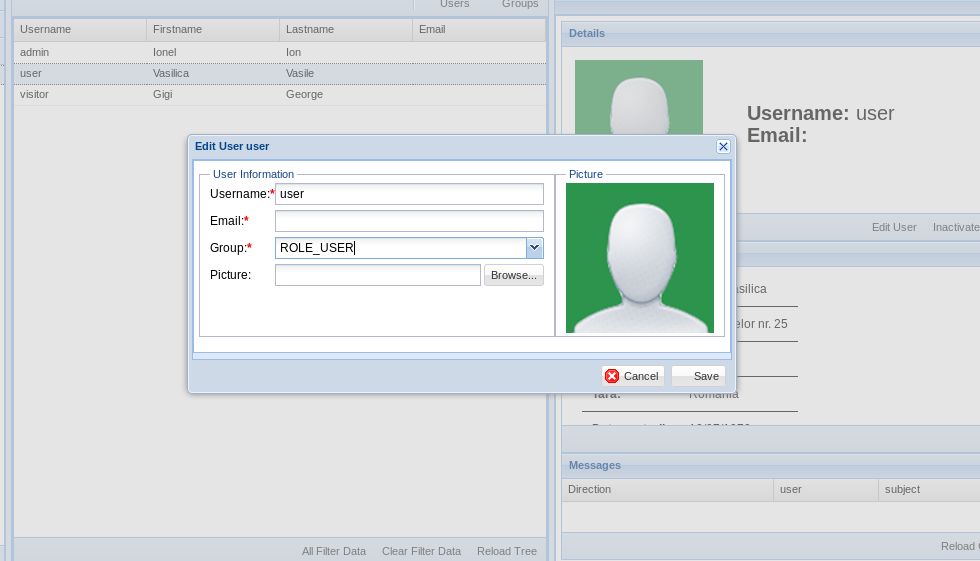
\includegraphics[width=10cm]{user/user2}

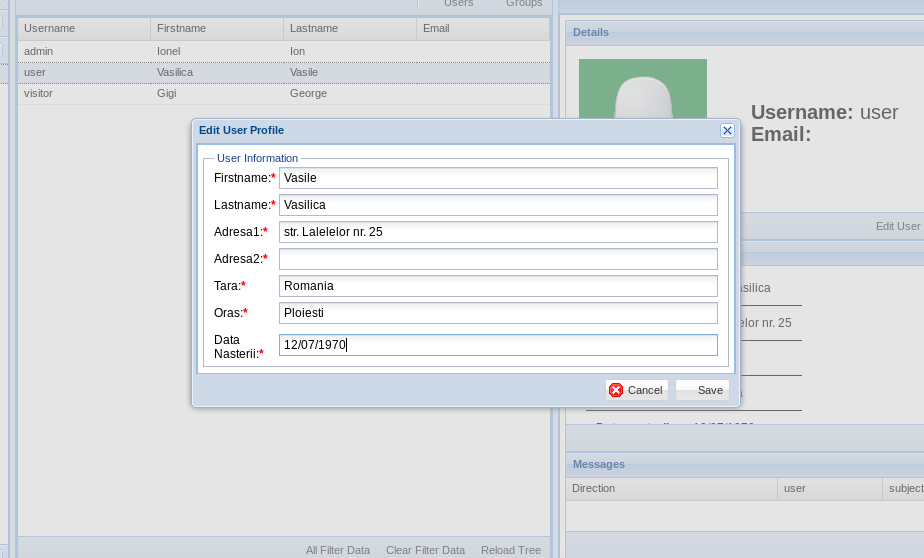
\includegraphics[width=10cm]{user/user3}

Modulul permite de asemenea modificarea proprietatilor grupurilor.

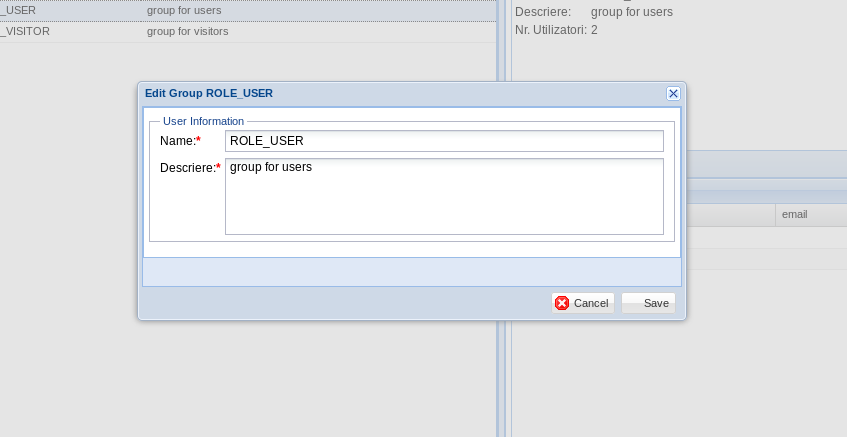
\includegraphics[width=10cm]{user/user5}

% Sorin

\chapter{Sistemul de jurnalizare}

\section{Interfata de administrare pentru sistemul de jurnalizare}

% Sorin - interfata

\subsection{Servicii de jurnalizare pe partea de server}

In etapa precedenta a proiectului a fost realizat sistemul de jurnalizare al aplicatiei. Detaliile referitoare la tehnologia folosita si la implementarea acesteia au fost descrise in anexa raportului corespunzator etapei a patra a proiectului.

Ulterior implementarii sistemului de jurnalizare, au fost dezvoltate controller-e si servicii care permit obtinerea de informatii relevante in urma procesului de audit. Un scop important al noilor clase dezvoltate il constituie furnizarea acestor date interfetei de administrare a aplicatiei, pentru o buna monitorizare a activitatii care se va desfasura pe platforma RODA.

Controller-ele dezvoltate permit lansarea de cereri sub forma URL-uri de mai jos:

\begin{itemize}
\item{/admin/revised-objects - furnizeaza lista obiectelor care au aparut in cadrul reviziilor asociate procesului de audit al aplicatiei}
\item{/admin/revised-users - furnizeaza lista utilizatorilor (campul username) care au efectuat revizii}
\item{/admin/revised-dates - furnizeaza lista datelor calendaristice la care s-au efectuat revizii}
\item{/admin/revisions[/{revision}] - furnizeaza informatii asupra tuturor reviziilor daca partea optionala a URL-ului nu este prezenta, respectiv asupra reviziei avand identificatorul egal cu valoarea lui fragmentului revision din URL, in caz contrar.}
\item{/admin/revisions-by-date[/{date}] - furnizeaza informatii despre revizii, grupate dupa datele la care acestea au avut loc. Daca fragmentul date al URL-ului este prezent, se obtin informatii despre reviziile desfasurate la data respectiva. In particular, in interfata este utila folosirea controller-ului corespunzator lui /admin/revised-dates, pentru obtinerea tuturor datelor posibile, urmata de selectarea unei date din lista returnata. Pentru data respectiva, are loc invocarea acestui controller si obtinerea informatiilor despre reviziile corespunzatoare ei.}
\item{/admin/revisions-by-object[/{object}] - furnizeaza informatii despre revizii, grupate dupa obiectele asupra carora acestea au avut loc. Daca fragmentul object al URL-ului este prezent, se obtin informatii despre reviziile in care au avut loc modificari asupra obiectului respectiv. In particular, in interfata este utila folosirea controller-ului corespunzator lui /admin/revised-objects, pentru obtinerea tuturor obiectelor posibile, urmata de selectarea unui obiect din lista returnata. Pentru obiectul respectiv, are loc invocarea acestui controller si obtinerea informatiilor despre reviziile care au l-au afectat.}
\item{/admin/revisions-by-user[/{username}] - furnizeaza informatii despre revizii, grupate dupa utilizatorii care le-au efectuat. Daca fragmentul username al URL-ului este prezent, se obtin informatii despre reviziile efectuate de catre utilizatorul respectiv. In particular, in interfata este utila folosirea controller-ului corespunzator lui /admin/revised-users, pentru obtinerea tuturor utilizatorilor posibili, urmata de selectarea unui utilizator din lista returnata. Pentru utilizatorul respectiv, are loc invocarea acestui controller si obtinerea informatiilor despre reviziile pe care le-a efectuat.}
\item{"/admin/revisionsinfo[/{revision}] - furnizeaza informatii complete asupra tuturor reviziilor daca partea optionala a URL-ului nu este prezenta, respectiv asupra reviziei avand identificatorul egal cu valoarea lui fragmentului revision din URL, in caz contrar. In particular, in interfata este utila folosirea controller-ului corespunzator lui /admin/revisions, pentru obtinerea tuturor reviziilor posibile, urmata de selectarea unei revizii din lista returnata. Pentru revizia respectiva, are loc invocarea acestui controller si obtinerea informatiilor referitoare la obiectele, liniile si coloanele modificate, data reviziei, precum si utilizatorul asociat ei.}
\item{/admin/simple-revisions-by-object[/{object}[/{id}]] - furnizeaza informatii generale (simplificate) asupra reviziilor desfasurate asupra tuturor obiectelor (daca nu este specificata partea optionala a URL-ului), asupra unui singur obiect (daca este specificat fragmentul object din URL) sau asupra unei linii a unui obiect (daca sunt specificate atat fragmentele object si id).}
\item{/admin/simple-revisions-by-user[/{username}] - furnizeaza informatii generale (simplificate) asupra reviziilor desfasurate de catre fiecare utilizator daca partea optionala a URL-ului nu este prezenta, respectiv asupra reviziilor efectuate de catre utilizatorul corespunzator valorii din fragmentului username din URL, in caz contrar.}
\end{itemize}





% Letitia - serviciile implementate, legate de audit

\end{document}
